\begin{frame}{My research work}

Question: How do cities emerge, grow, and \textit{compete} over space?
\begin{figure}
    \centering
    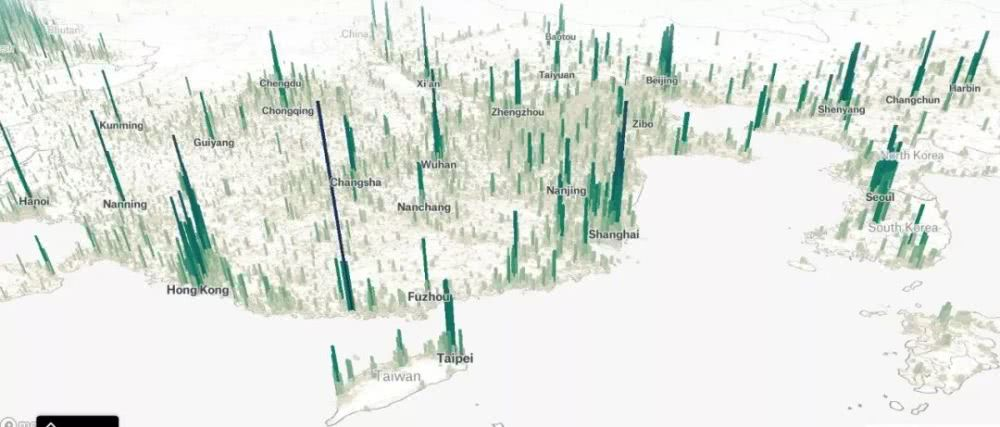
\includegraphics[width = 0.8\textwidth]{Pics/Population_hight_real.jpeg}
    \caption{Population distributions of Eastern China and the Korean Peninsula. \href{https://new.qq.com/rain/a/20190129A06G9C}{\textit{Source link}}}
    \label{fig:pop_real}
\end{figure}
\end{frame}

\subsection{Whys}
\begin{frame}{Why is it important, and what have and haven't been done?}
    % 分成三页ppt。
    Urbanization is complex and diverse, but scaling laws are similar.
    \vspace{0.5cm}
    
    Obvious basic rules behind cities:
    \begin{itemize}
        \item Zipf's law
        \begin{itemize}
            \item The rank size distributions of cities follow a specific form:$P(n) \sim n^{-(1+\gamma)}$, where $\gamma\approx 1$.
        \end{itemize}
        \item Clark's Law
        \begin{itemize}
            \item The spatial distributions of population within a city exponentially decay from urban center: $p(r) \sim P_0e^{-\alpha r}$.
        \end{itemize}
        \item Fractality
        \begin{itemize}
            \item Urban envelopes are fractal.
        \end{itemize}
    \end{itemize}
    
    % Is Zipf's law the same everywhere?
    \begin{center}
        \only<1>{}
        \only<2>{\textbf{How to model? }}
    \end{center}
\end{frame}

\begin{frame}{Why is it important, and what have and haven't been done?}
% 跟上面第一点结合起来
    Existing models have explained the empirical results of Zipf's, Clark's, and scaling laws.
    \begin{itemize}
        \item migration patterns\cite{PhysRevLett.120.108701},
        \item spatial gathering\cite{Li2017Simple}, 
        \item reaction-diffusion\cite{marsili1998interacting}, 
        \\ ......
    \end{itemize}
    Leading to asymptotic behavior of Zipf's law. 
    
    \vspace{0.5cm}
    \begin{center}
        \only<1>{\textbf{Emerge? Grow? Compete?}}
        \only<2>{\textbf{Emerge? Grow? \sout{Compete?}}}
    \end{center}
    
\end{frame}

\begin{frame}{Observations}
Urbanization won't last forever. It is also not driven by pure growth dynamics. It has its own critical dynamics in the percentage of resource. It also has temporal advantages. \textbf{Cities are competitive.}
    \begin{figure}
        \centering
        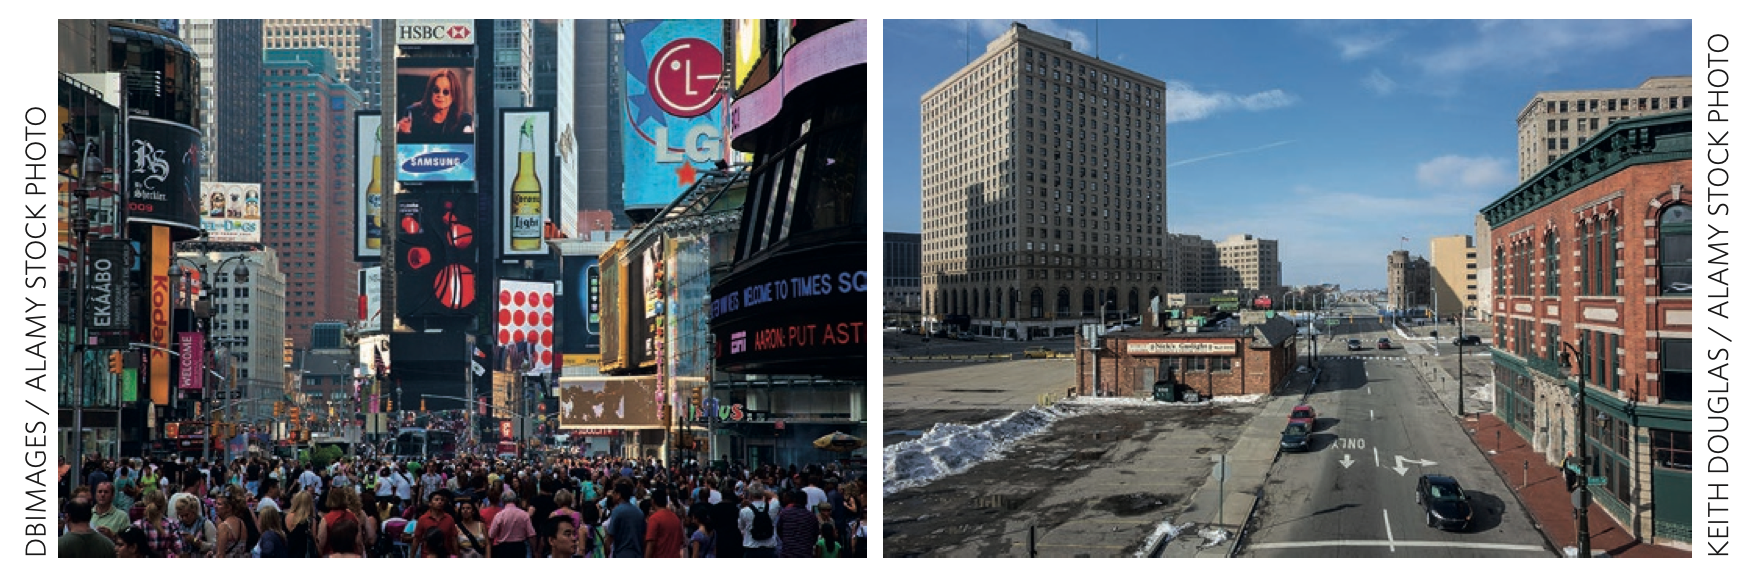
\includegraphics[width = 1\linewidth]{Pics/batty_nyc_detroit.png}
        \caption{NYC \& Detroit. From Michael Batty's thesis, \textit{Diverse cities, successful cities}\cite{batty2017urban}.}
        \label{fig:batty's}
    \end{figure}
    \begin{center}
    \only<1>{Economic complexity and cultural evolution}
    \only<2>{\textbf{We want it simpler.}}
    \end{center}
\end{frame}

\subsection{Formations}
\begin{frame}{Philosophy}
\textbf{Competition for Resource}
    \begin{itemize}
        \item Cities grow because they are \textbf{competitively} better (than rural area or other cities).
        \item The \textbf{total competitiveness} lies in the \textbf{finite active population} $\equiv N^*$.
        % like the IT guys or financial practitioners.
        \item Active people either:
        \begin{itemize}
            \item move in cities and settle somewhere, driven by other actives' attraction, (with rate $\beta_2$);
            \item or establish a new city, (with rate $\beta_1$).
        \end{itemize}
%         \item Active population can be interpreted
% as the people who serve in information industry or finance markets. 
    \end{itemize}
    \begin{center}
        \textbf{Rank relevant intellectuals?}
    \end{center}
\textbf{Competition for Space}
    \begin{itemize}
        \item Once a site is occupied by a city, you can settle here only if you belong here.
    \end{itemize}
\end{frame}

\begin{frame}{Model}
    \begin{figure}
        \centering
        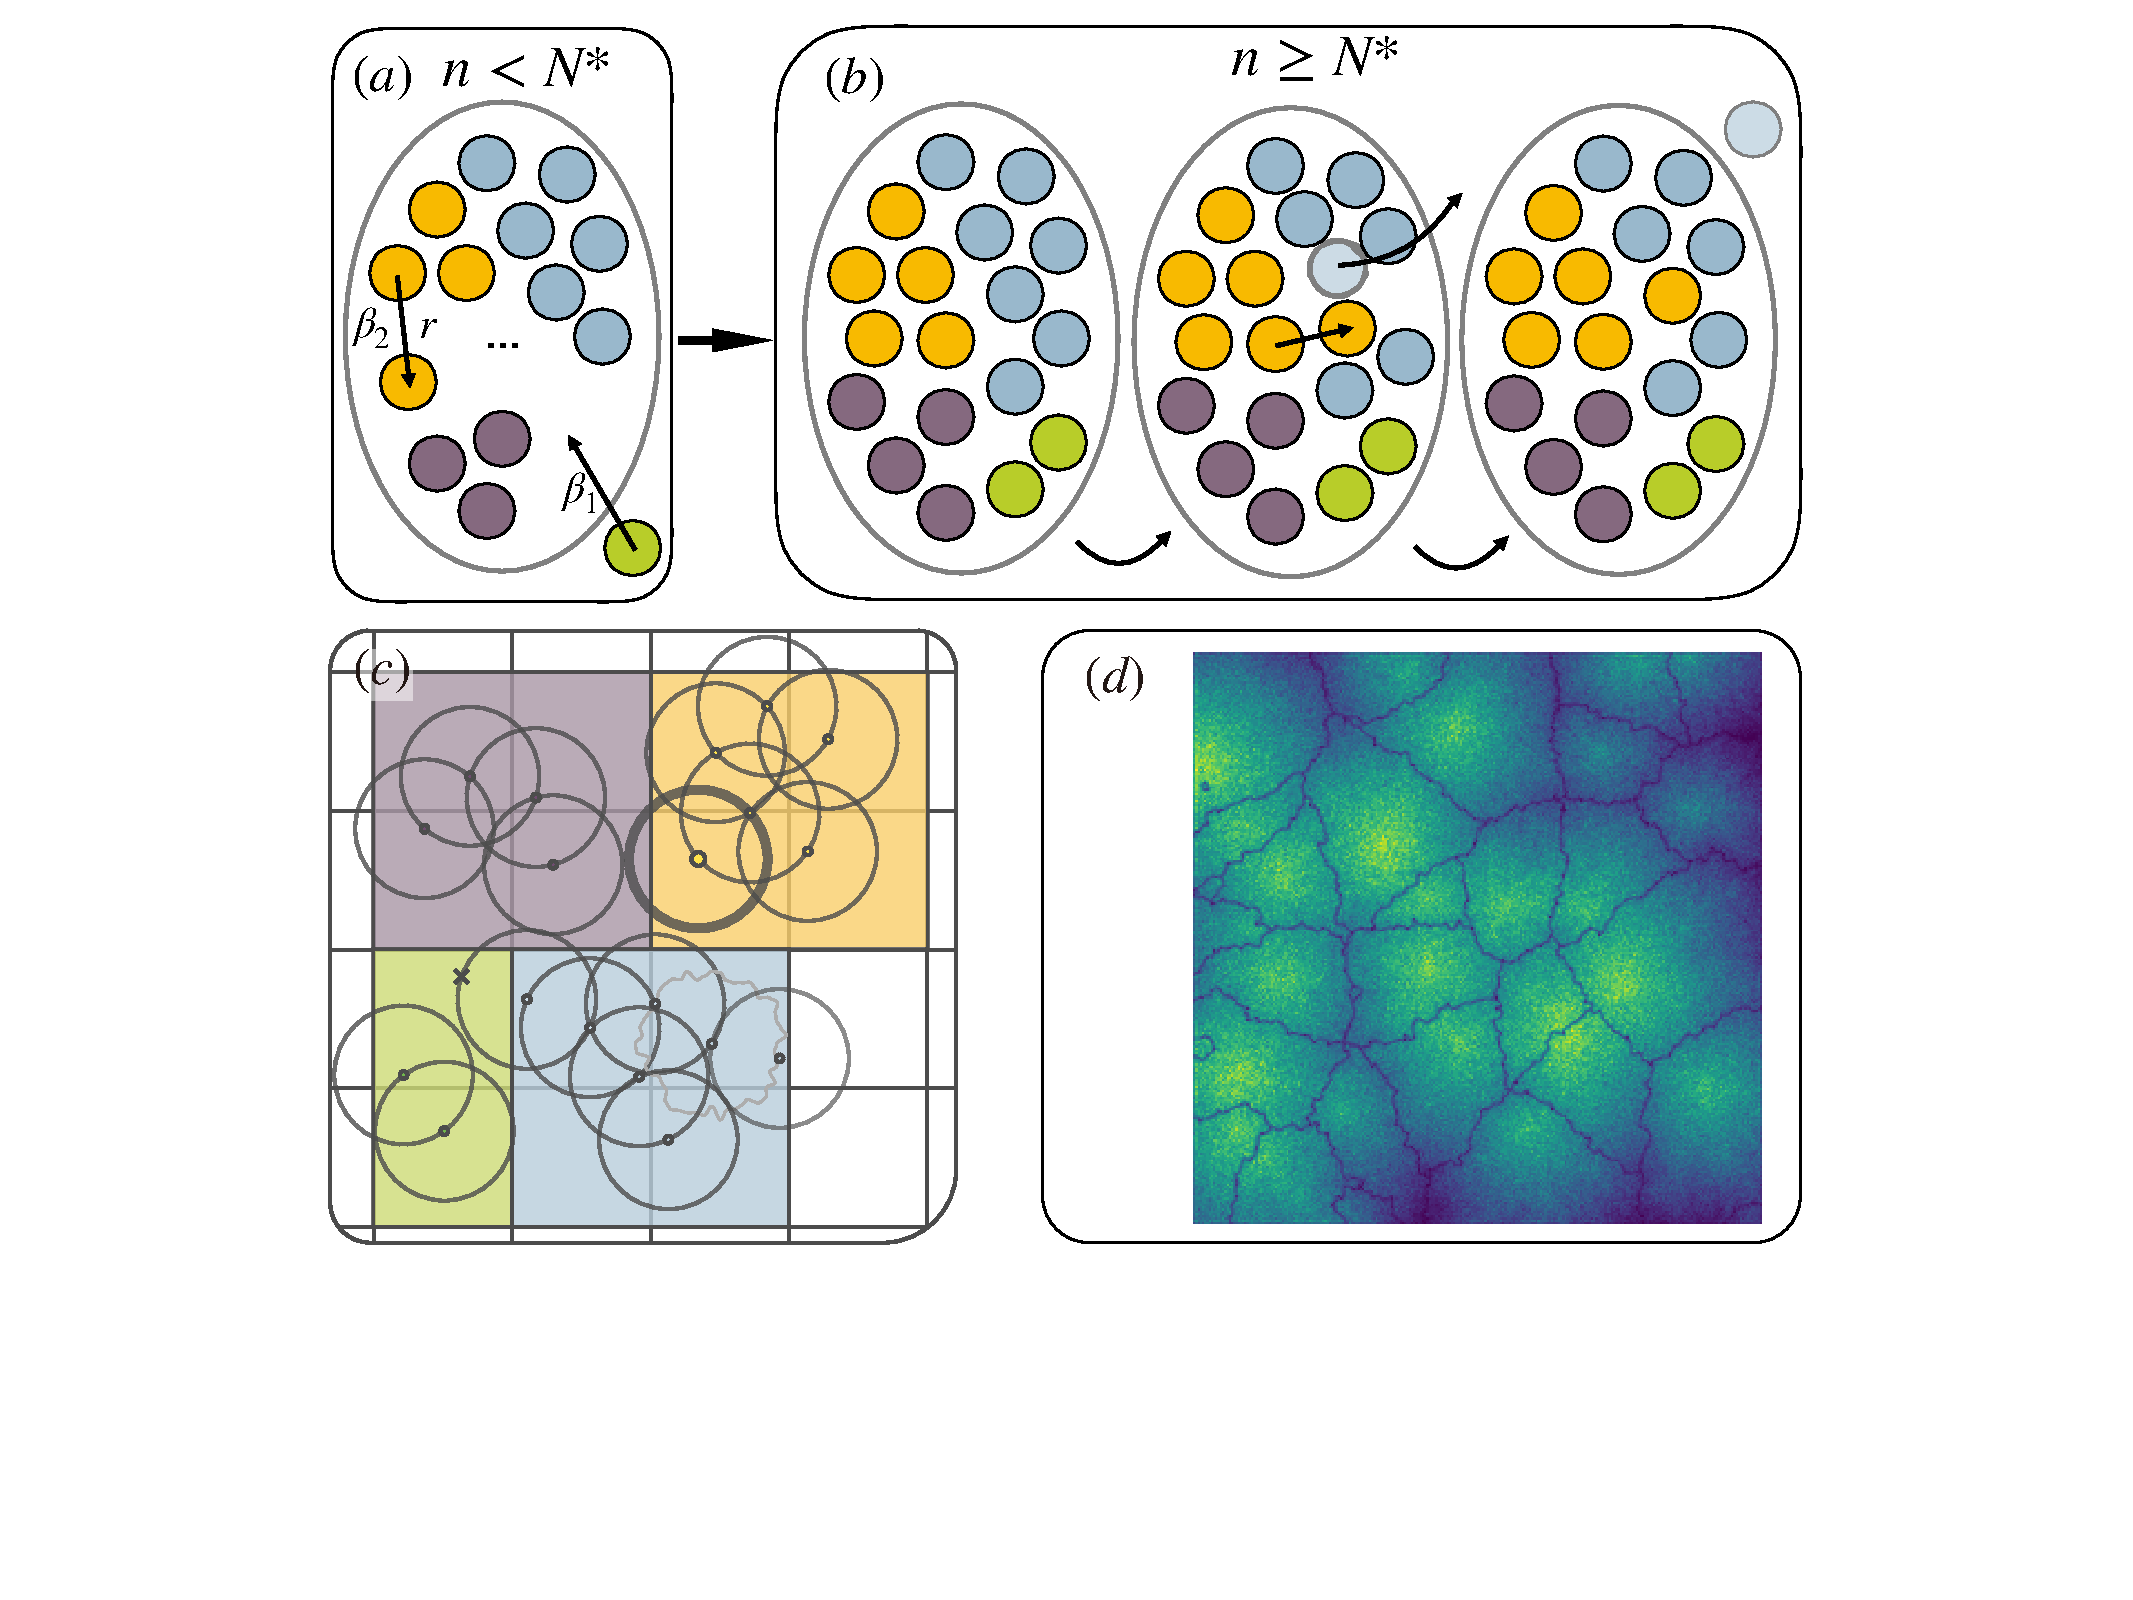
\includegraphics[width = 0.8\linewidth]{Pics/sketchgood.pdf}
        \caption{Model sketch: (a) Speeds of additions of \# of cities and citizens; (b) The role of the memory kernel; (c) Spatial settings; (d) A realization with $\beta_1 = 0.25$, $\beta_2 = 1$, $r=0.5$, $N = 10^5$. }
        \label{fig:sketch}
    \end{figure}
\end{frame}
\begin{frame}{Model}
    \textbf{Notions:}\\
    \hspace{0.25cm}$N_i(t)$: \# of active citizens in $i$'th city at time $t$;\\ \hspace{0.25cm}$k(t)$: \# of cities at time $t$.\\
    \textbf{Rules:}
    \begin{itemize}
        \item The model is based on continuous space and time context.
    \item Growth: restricted preferential attachment. 
    \begin{itemize}
        \item $dN_i(t)/dt = \beta_2 N_i(t) -\delta_{\{\sum N_i = N^*\}} \beta_1k(t)$\\ \hspace{1.8cm}$-\delta_{\{\sum N_i = N^*\}} (N^*-N_i(t))\beta_2$,
        \item $dk(t)/dt = \beta_1k(t)$.
    \end{itemize}
    
    \item Spatial settings:
    \begin{itemize}
        \item Grid blocks. Once a block is taken by one city, citizens from other cities cannot survive.
        \item New city: uniformly, if empty? confirmed.
        \item New active citizen: $(r,\theta)$ from an existing active citizen.
    \end{itemize}
    \item \textit{All parameters:} $r$,$\beta:=\beta_2/\beta_1,$
    \end{itemize}
\end{frame}

\subsection{Results}
\begin{frame}{Results: As an urban system}
    \begin{figure}
    
        \centering
        \begin{minipage}{0.48\linewidth}
        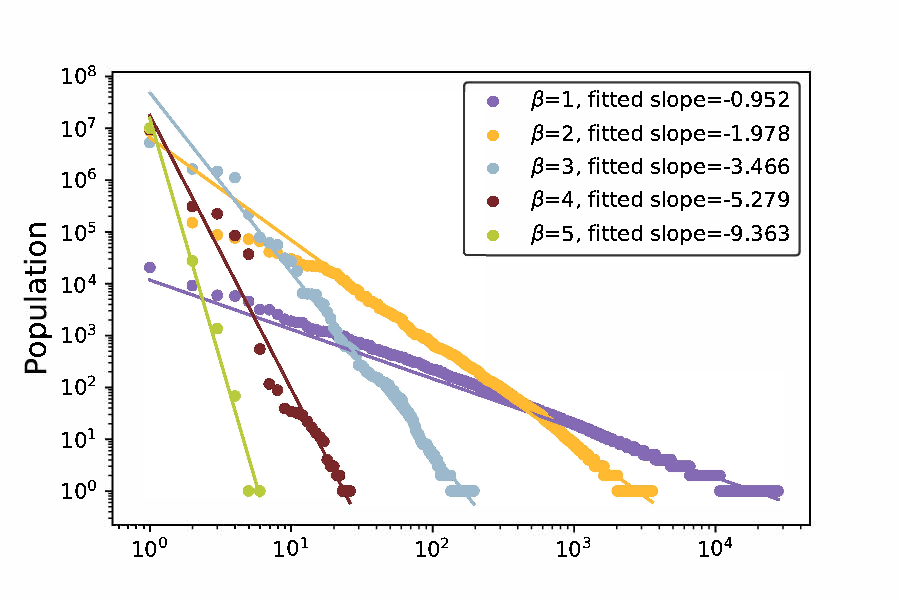
\includegraphics[width = 0.9\linewidth]{Pics/zipf.pdf}
        \caption{Zipf's law of rank size distribution; $\beta:=\beta_2/\beta_1$}
        \end{minipage}
        \begin{minipage}{0.48\linewidth}
        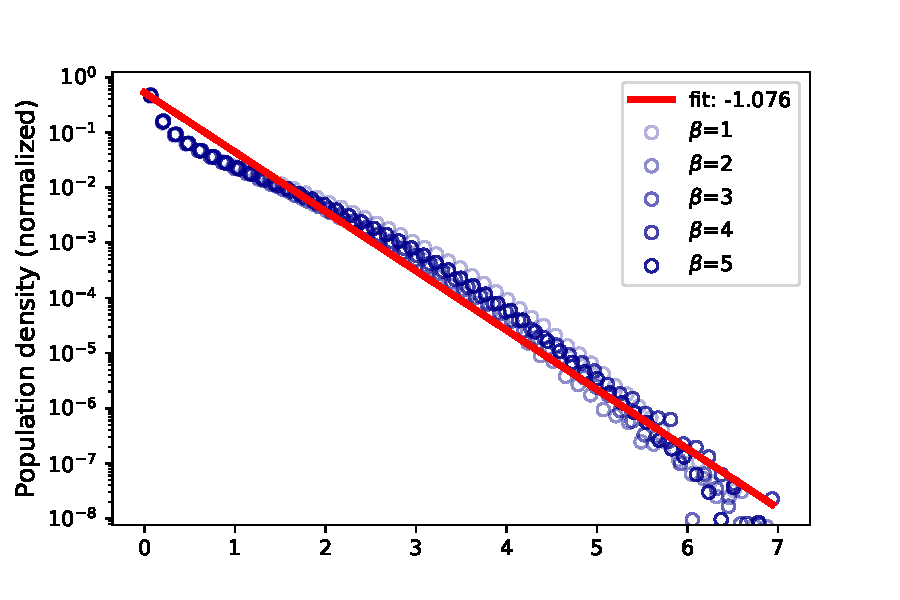
\includegraphics[width = 0.9\linewidth]{Pics/kernal_density.pdf}
        \caption{Clark's law for a city's population density.}
        \label{fig:Zipf}
        \end{minipage}
    \end{figure}
    
    \textbf{SYM is a successful model for urban systems that reformulates Zipf's and Clark's law.}
\end{frame}

\begin{frame}{Results: Competitions for \textbf{resource} and space}
    \textbf{Critical density:}
    \[\rho_{threshold} = k/\beta.\] $\uparrow$ with \# of cities $k$. Survival probability of a site $\downarrow$.
    
When the space is filled, \textbf{Critical population:}
    \[N_{threshold} = 0.5 N^*\]
\textbf{Turnover rate:}
\begin{figure}
    \centering
    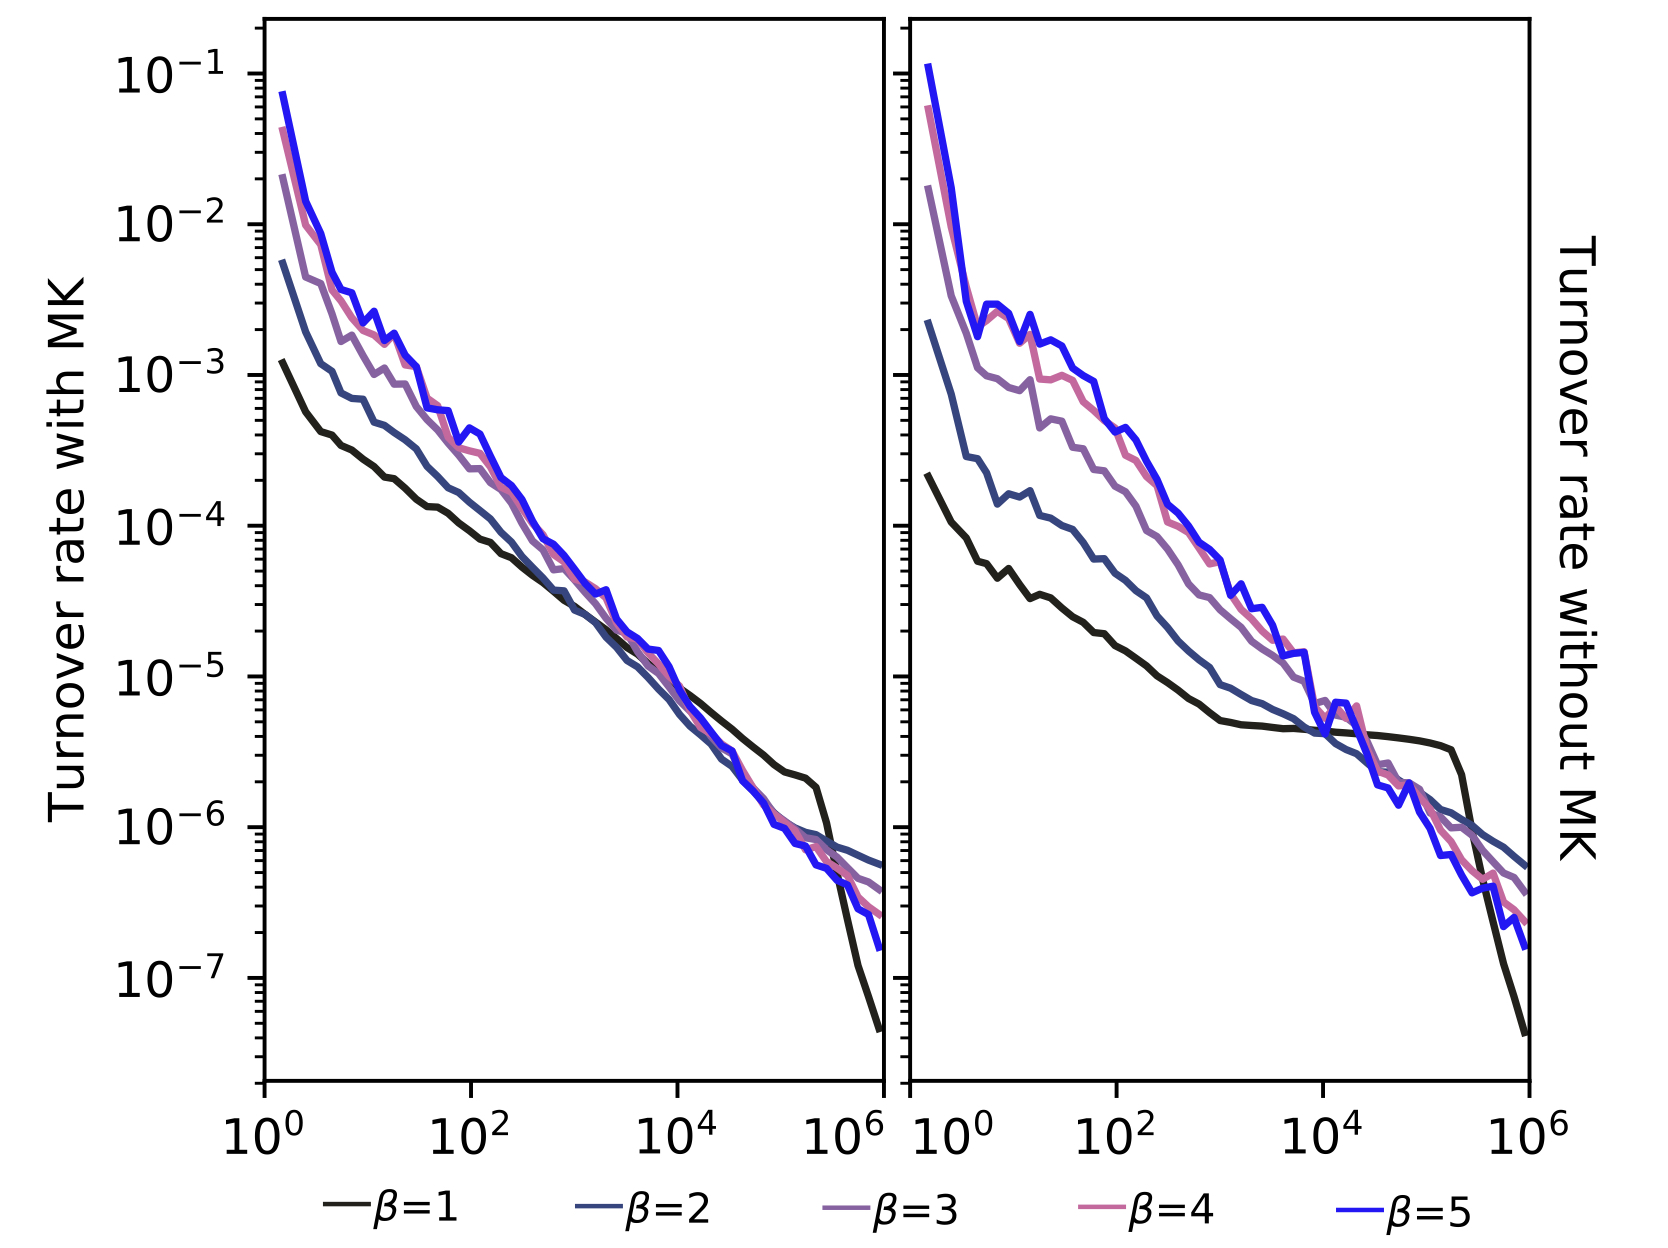
\includegraphics[width = 0.65\linewidth]{Pics/in_one.jpeg}
    \label{fig:turnover}
\end{figure}

\end{frame}

% \begin{frame}{Results: Competitions for resource and \textbf{space}}

% \begin{figure}
%     \centering
%     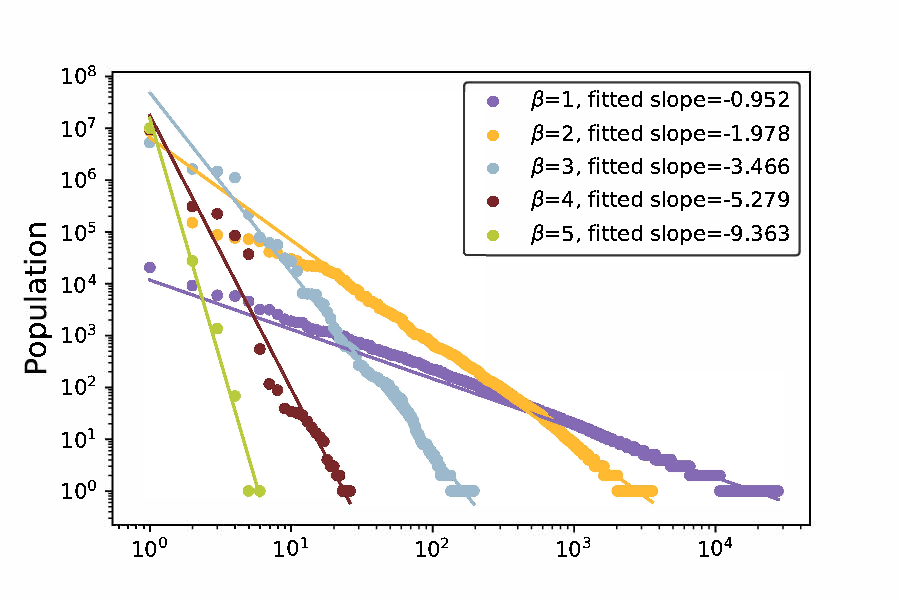
\includegraphics[width = 0.9\linewidth]{Pics/zipf.pdf}
%     \caption{Zipfian exponents are significantly larger when $\beta\uparrow$.}

% \end{figure}
    
% \end{frame}

\begin{frame}{Results: Competitions for resource and \textbf{space}}
\begin{minipage}{0.6\linewidth}
\begin{figure}
    \centering
        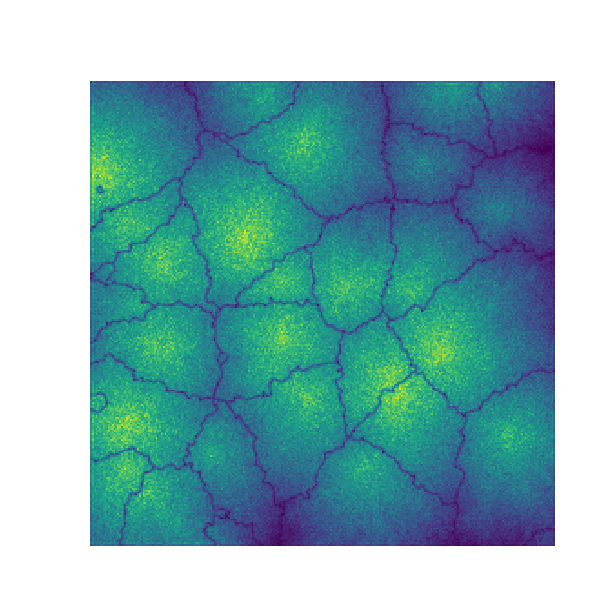
\includegraphics[width = 0.6\linewidth]{Pics/fractal_41_256.pdf}
        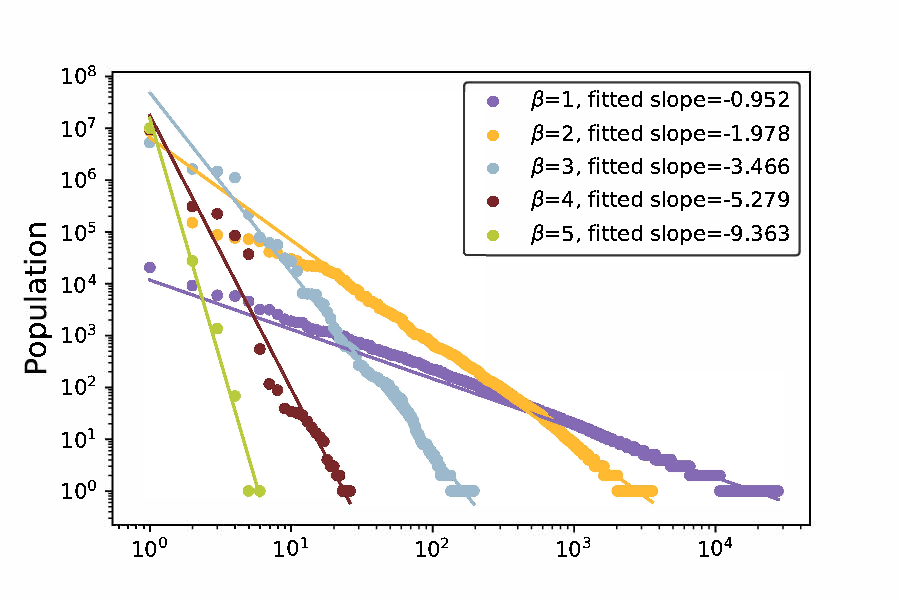
\includegraphics[width = 0.6\linewidth]{Pics/zipf.pdf}
        \caption{\textit{Above:} Fractal edges drawn from SYM. \textit{Below:} The absolute values of the slopes are expected as $\beta$ without a spatial context.}
    
    \label{fig:my_label}
\end{figure}
\end{minipage}
\begin{minipage}{0.38\linewidth}
\begin{itemize}
    \item Small cities are advantageous for spatial competitions.
    \item For large $\beta$'s, the survival probability of small cities decreases rapidly, bring advantages for big cities.
\end{itemize}
\end{minipage}

\end{frame}

\begin{frame}{Our histogram}
    \begin{figure}
        \centering
        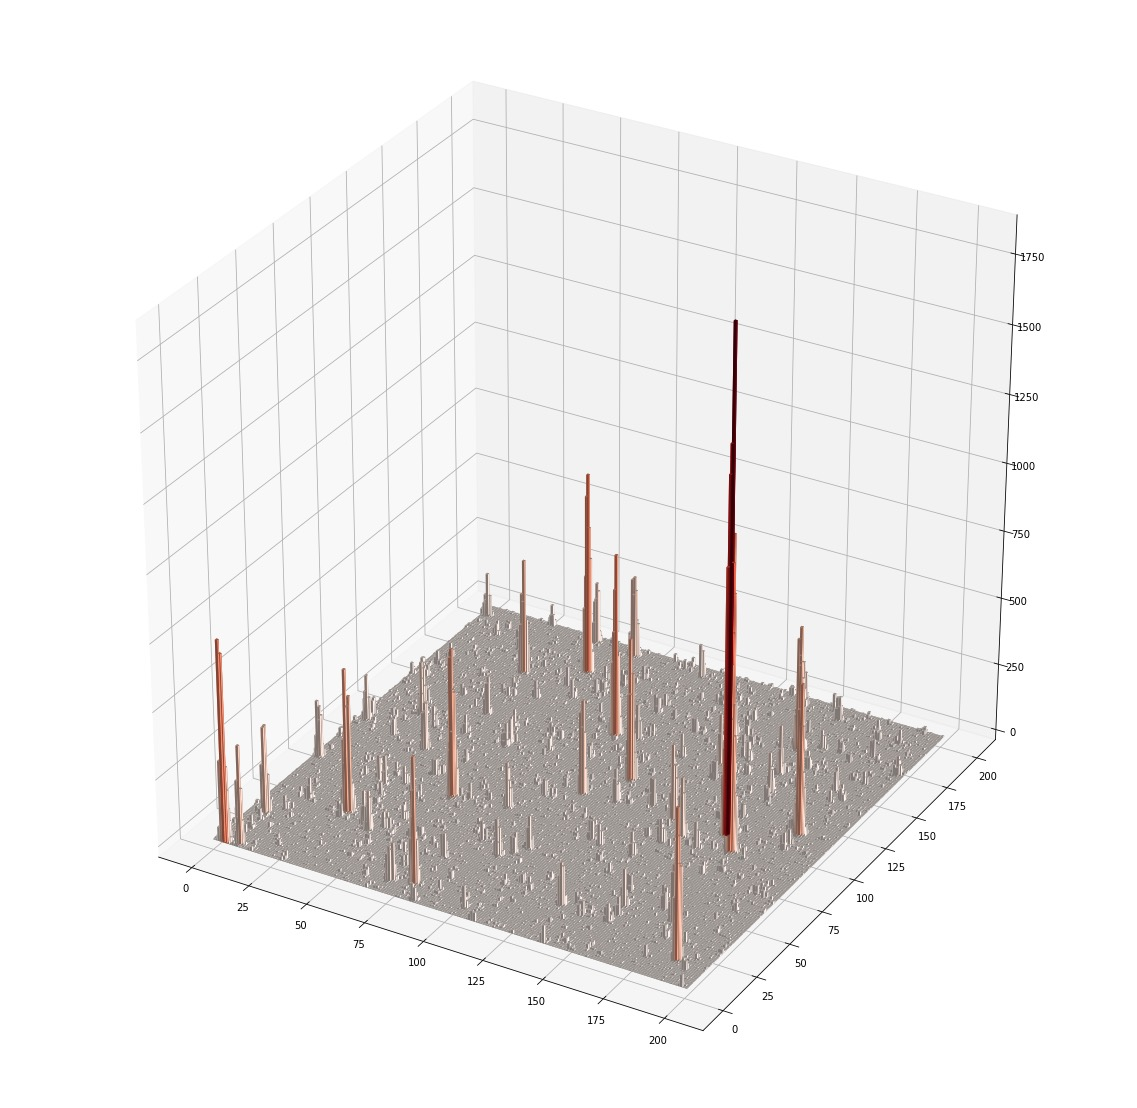
\includegraphics[width = 0.7\linewidth]{Pics/3dhist.jpeg}
        \caption{Simulated result.}
        \label{fig:my3dhist}
    \end{figure}
\end{frame}
\subsection{Insights}
\begin{frame}{Insights}
    \begin{itemize}
        \item The tendency of vicissitudes is strengthened by the restrictions of resource. \item The bottom-up formations of traditional models are not enough to model cities.
        \item Zipf's law with $\gamma \approx 1$?
            \textbf{Not quite!}
        \item Spatial competition has to be taken serious, especially for small areas. 
        \item Critical phenomena from branching process can be broadly adopted.
    \end{itemize}
\end{frame}